\documentclass[11pt, a4paper]{article}
\usepackage{opgave}
\usepackage{fancyStyle}
\usepackage{hyperref}
\usepackage{listings}

\renewcommand{\course}{DEV01-1}
\renewcommand{\titel}{Assignment 4}
\renewcommand{\auteur}{The INFDEV Team @ HR}
\renewcommand{\auteurlang}{\auteur}

\setboolean{isTentamen}{false}
\setboolean{showAntwoord}{false}

\usepackage{graphicx}

\begin{document}
\setcounter{opgave}{1}
This is the first of the three assignments that will be graded.
You can score a maximum of $3$ points for this assignment, 1 point for each exercise.
For every sub-assignment, write a program in it's own separate file.

\opgave{Warmup}{1}
\subopgave{Write a program that asks for a users input, converts Fahrenheit to Celcius and shows the amount of Celsius with a precision of 2 decimals.
You can ask a user for input using:
}{}{1}
\lstset{language=Python, showstringspaces=false}
\begin{lstlisting}
  age = input("What's your age?")
\end{lstlisting}


\subopgave{Write a program that converts Celcius to Kelvin. Also handle absolute zero in a clean manner.}{}{1}
\subopgave{Write a program that calculates the absolute value of a number. That is, the absolute value of $-15$ is $15$,
 the absolute value of $10$ is $10$, etc.}{}{1}

\opgave{RPS}{1}
 \subopgave{Write a program for the game Rock, paper, scissors. The program should:
  \begin{itemize}
   \item ask the users to write down their choice,
   \item tell what happens (Scissors cut paper) and
   \item tell who won (player 1 wins)
  \end{itemize}
  }{}{0}
 \subopgave{Extend your rock-paper-scissors program into rock, paper, scissors, lizard, spock. Don't know what that is? Look at this explanation: \href{https://goo.gl/gisNA8}{goo.gl/gisNA8}
 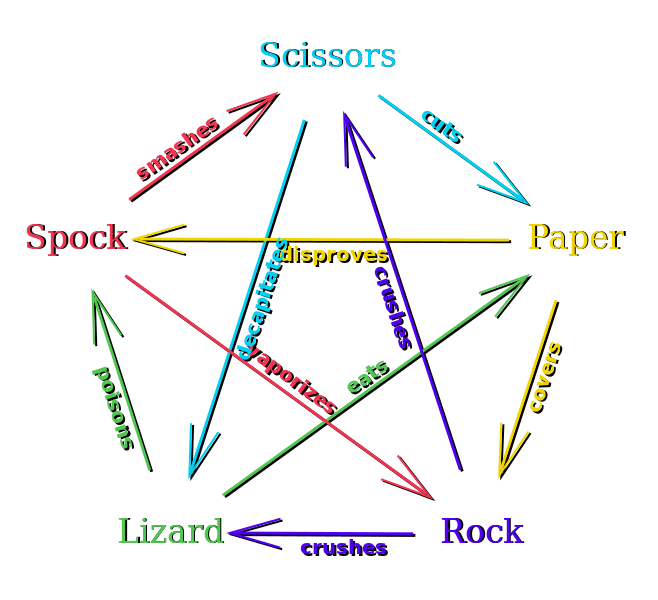
\includegraphics[width=6cm]{658px-Rock_Paper_Scissors_Lizard_Spock_en.svg.png}
 }{}{0}

\opgave{Turtle}{1}
 \subopgave{Turtle graphics is a popular way to introduce programming to kids. It was part of the original Logo programming language developed by Wally Feurzig and Seymour Papert in 1966. For this assignment write \textbf{a program that controls the movement of a turtle}. Specifically the program should:
 
 \begin{itemize}
 \item Move the turtle forward by an 'amount' of steps (find a proper amount) when the user presses the key W,
 \item Turn the turtle by 'amount' of degrees (find a proper amount) when the user presses the key A or D, and
 \item Provide at least one behavior (free-choice) that is implemented by mean of one or more if's 
 \end{itemize}

 
We provide you a project in Visual Studio 2015\footnote{For those who wants to use a different IDE copy the files Start.py, Program.py, and End.py into your project. Mind to run run first Program.py} that contains several files. Follow the instruction in the file called \textit{Program.py}. The project is available in the folder called Turtle on Natschool. 
 }{}{0}



\einde
\end{document}